% Andrew G. West - prop_spec.tex
% Main LaTeX file for CIS400/401 Project Proposal Specification
%

\documentclass{sig-alternate}
 
\usepackage{mdwlist}
\usepackage{url}
\usepackage{graphicx}
\usepackage{float}
\usepackage[section]{placeins}
\begin{document} 

\title{BERTRAM: A Bartending Robot}

\subtitle{Dept. of CIS - Senior Design 2011-2012}
\numberofauthors{3}
\author{
\alignauthor Seth Shannin \\ \email{sshannin@seas.upenn.edu} \\ Univ. of Pennsylvania \\ Philadelphia, PA
\alignauthor Kevin Xu \\ \email{kevinxu@seas.upenn.edu} \\ Univ. of Pennsylvania \\ Philadelphia, PA
\alignauthor Dr. Camillo Jose Taylor \\ \email{cjtaylor@cis.upenn.edu} \\ Univ. of Pennsylvania \\ Philadelphia, PA}
\date{}
\maketitle

\begin{abstract}
\textit{\indent Programming a robot to autonomously perform human tasks has been a 
long-time goal of robotics. Such endeavors have typically involved heavy 
computation due to the demands of visual processing, path planning, and motor 
coordination. Human demonstration has often been used to introduce a sequence 
of moves to a robot, both in the form of direct physical manipulation of the 
robot and translating information from visual motion capture. Here we 
investigate teaching robotic motion through the development of an immersive
teleoperation system for controlling the PR2. Unlike previous attempts to
control the PR2 from a distance (`teleoperation'), we propose to also provide the
operator with an `immersive' experience by allowing the operator to experience the robot's
environment from the robot's perspective. We plan to evaluate the effectiveness of the system
by attempting to mix and serve drinks with a Willow Garage PR2 
humanoid robot controlled by a user of this immersive teleoperation system.
\\\indent Following the implementation of this system, we will then evaluate how the system can be used to allow
the PR2 (or any robot for that matter) to rapidly acquire and refine different complex behaviors within a specific environment. If successful, we will have demonstrated a novel and easy way for a
human operator to impart a specific movement sequence on to a robot. This paper details our progress in regards to implementing the immersive teleoperation system and our plans to teach the PR2 with it.}
\end{abstract}

	% AW - Then we proceed into the body of the report itself. The effect of the 'section' command is obvious, but also notice 'label'. Its good practice to label every (sub)-section, graph, equation etc. -- this gives us a way to dynamically reference it later in the text via the 'ref' command.
\section{Introduction}
\label{sec:intro}
\indent Constructing a fully autonomous and adaptive robot has been a long-time goal of robotics research.
The possibility of a robotic butler is only one of many potential applications. However, real
autonomous decision making (that is, free of direct control from a human operator) is an incredibly challenging process, for many different processes must 
be coordinated to make this possible. For instance, vision processing must be done quickly and accurately to respond to 
changes in the environment, accurate path planning is needed to navigate the environment, and 
precise motor coordination is needed to manipulate the environment. There have been many different 
attempts at overcoming these challenges involved in developing an autonomous robot. One major type of approach 
that has been often explored involves the field of machine learning. The ability to learn can be a powerful intermediate 
step towards autonomy, since learning can allow a robot to adapt to new, unforeseen scenarios on its own. 
Teaching by human demonstration is a common approach to robot learning since it enables the 
transmission of complex behavior in a manner far easier than individually planning the movement of each motor and joint. However, choosing how exactly how the demonstrated behavior is delivered to the 
robot in such a way that it can record and reproduce that behavior is still a very challenging task.\\ 
\indent In this paper we report on our progress towards teach the WillowGarage PR2 Robot how to mix and
serve drinks by first implementing an immersive teleoperation system for controlling the PR2. By `teleoperation', we simply mean control from
a distance. By `immersive', we mean giving the human operator the illusion of being inside the PR2. The PR2 is a humanoid robot developed by  Willow Garage~\cite{pr2} for the purpose of robotics 
research. It is omnidirectional and capable of telescoping height. What makes the PR2 especially attractive for robotics research is its pair of highly movable arms and grippers that allow grasping of many different kinds of objects. The PR2 also comes with a robust series of highly useful software development tools,
including a versatile simulator that allows developers to perform trial runs on a virtual PR2 without
risking damage to the actual robot. Institutions across the world have taught the PR2 a wide variety of human actions, such as baking 
cookies~\cite{cookies}, scanning and bagging groceries~\cite{groceries}, and fetching a sandwich from 
Subway~\cite{subway}. However, unlike these examples, we propose to teach the PR2 a new behavior not through advanced task planning, but through human
demonstration. \\
\indent The chief component of our system is the Microsoft XBox Kinect sensor. This sensor provides depth information at real-time speeds
(30 frames per second), which essentially performs the computation that would have been required for stereo 
processing. Combined with various open source libraries~\cite{kinect}, the Kinect also works with 
software that provides human motion sensing and tracking, which greatly simplifies the task of capturing human body movements.
These Kinect libraries have already been used successfully in 
many projects involving real-time tracking of human motion, many examples of which can be found online~\cite{freenect}.\\
We propose to use the Kinect as part of an immersive teleoperation system to teach the PR2 how to mix and pour different kinds of drinks.
The Kinect sensor provides a convenient way to capture a human demonstration of desired behavior. The captured data can be relayed to the
PR2 via ROS, an open-source Robot Operating System\cite{ros}. ROS provides a convenient framework for inter-process communication and
coordination. Processes that perform computation are visualized as nodes in a graph, with inter-process communication representing the
edges of the graph. Nodes send information to each other in the form of messages. Nodes that wish to send messages to other nodes can
'publish' to a topic, and nodes wishing to receive these messages need only to 'subscribe' to these topics. ROS enables relatively short
programs to issue surprisingly sophisticated commands to the PR2, such as moving all of the arm joints to a specific position within a
specified time frame. By using ROS along with the PR2 and the Kinect, we will construct a system for operating the PR2 remoting while
giving the operator the feeling of being within the robot itself. We will then evalute the effectiveness of this system in teaching the PR2 new tasks.\\
\indent Our method has several advantages over existing approaches. First of all, the Kinect sensor provides accurate real-time human
motion tracking that can be mapped to specific movement in the PR2 thanks to ROS. Secondly, an immersive scheme for controlling the robot
enables a human operator to more naturally move the robot in a given situation compared to manipulating the robot directly by physical
contact or through a joystick-based control scheme. Immersive teleoperation also enables direct control of robots that cannot be easily
subject to demonstration through physical contact, such as very large or very small robots. Our method, if successful, would allow for rapid demonstration of different sequences of behavior to the PR2, which could be stored and queued up for later reproduction. This technique could be generalized to other humanoid robots besides the PR2 to teach them different kinds of behavior.\\
\indent This paper will first outline the components of the system before delving into the technical implementation of each component. Following that will be an evaluation of the current performance of the system and a summary of remaining work.	
\section{Related Work}
\label{sec:related_work}
Other institutions have conducted research involving autonomous robots and handling drinks. Hillenbrand \textit{et al.}~\cite{pouring_arm} designed a semi-autonomous hand-arm robot for serving drinks. The hand-arm was capable of responding to user input by choosing a drink from a variety of different containers, opening the drink if necessary, pouring the liquid into a glass, and then offering the drink to the user. It was capable of not only picking up bottles and cups, but also of unscrewing bottle caps. Stereo processing was combined with object recognition to identify the drinks, after which grasp planning was used to actually pick up and manipulate the drink. Srinivasa \textit{et al.}~\cite{herb} designed an autonomous robot capable of navigating a household-like environment and manipulating a wide variety of everyday objects. Consisting of an arm mounted on a segway, HERB used a powerful array of six multi-core processors to successfully traverse its environment and interact with objects around it, such as cups and drawers. By combining modules for object recognition, task based planning, caged grasping, and workspace goal regions, HERB was able to autonomously carry out commands issued from a GUI to perform simple kitchen tasks such as placing an object in a recycling bin.\\
There has also been substantial work done in teaching the PR2 robot to perform human tasks. Bohren \textit{et al.}~\cite{beer} used the PR2 and ROS to build a robotic system for retrieving a beer from a refrigerator. In their work, they developed a task-level execution system known as SMACH for rapidly prototyping robotic applications. The PR2 had to navigate an obstacle map to reach the refrigerator, use object recognition and grasp planning to identify the door handle and the drinks, and ultimately use facial recognition to deliver the beer to a human recipient. Each step of the process contained detail planning and image processing in order to carry out the expected behavior. Klingbeil \textit{et al.}~\cite{groceries} developed a grasping algorithm to enable the PR2 to pick up objects and attempt to locate and scan the barcode. Their technique bypassed the training phase by allowing the PR2 to devise a plan to grasp the object from only a single 3D snapshot. Their algorithm emphasized the importance of positiong the PR2's gripper such that its shape most closely matched the shape of the object it attempts to grasp. Saito \textit{et al.}~\cite{subway} devised a method for the PR2 to intelligently navigate large environments via semantic search. The PR2 attempts to find a specific object by first searching areas that would logically contain that item. When asked to retrieve a sandwich, the PR2 first inspected a nearby refrigerator in its environment.\\ 
All of these robots relied on some combination of vision processing and path planning to carry out their tasks. However, there have been other approaches involving demonstration learning to allow a robot to perform a specific job. In a relatively early attempt, Chalodhorn \textit{et al.}~\cite{walk_imitation} used motion capturing to teach a bipedal humanoid robot how to walk by imitation. Joint angles from motion capture data from a human demonstrator wearing a motion capture suit were mapped to joint angles in the robot. This data was combined with predictions of future state based on sensory information to reproduce a human-like gait in the robot. Kormushev \textit{et al.}~\cite{whiteboard} taught a robot new motor skills through kinesthetic teaching. The robot had two distinct modes of operation: a learning phase and a reproduction phase. During the learning phase, the robot was shown how to clean a whiteboard by direct human manipulation of the robot's joints, recording both position and force information. During the reproduction phase, the robot would translate the learned information to its own reference frame and attempt to duplicate the teacher's movement pattern on the whiteboard.  Kormushev \textit{et al.}~\cite{pancakes} also used kinesthetic learning to teach a robotic arm how to flip a pancake. A human teacher first moved the arm to demonstrate the movement required to flip a pancake 180 degrees in the air and catch it again. In subsequent trials, reinforcement learning techniques were applied such that the robot could evaluate the performance of its flips and attempt to adjust the motion of the arm for better future flips.

\section{System Model}
Specifically because a teleimmersive system is meant to be used by human 
operators to control a robot, the external/visible part of this
design must be simple. The number of devices used to get input from the user 
and to deliver feedback should be small, and these devices should require
minimal effort to use. To that
end, a good portion of the control data captured from the user is captured
passively. After the initial setup phase, the user should be able to control
the system with minimal effort; the system should just watch the user and
translate the user's movements into control instructions for the PR2.

To facilitate this process, we use a couple separate devices and some
fairly sophisticated software stacks. While the
devices mostly consist of cameras and accelerometers to track the users 
motion, there are a couple handheld button devices to allow the user to
perform non-humanoid operations on the robot (such as freezing a joint or
triggering certain routines).

The true nexus of the system is ROS (Robot Operating System). Although the
user will never interact directly with ROS, all communication between the
user and the PR2 (in the form of commands or feedback) must pass through ROS.
ROS abstracts over devices and I/O, providing a common interface for accessing
any data stream or controlling any device. Using ROS, we can easily take
data from the many tracking devices, process all the data to come up with
movement plans for the PR2, and then actually command the PR2 to move in the
desired manner.

Other than the PR2 robot itself, the Microsoft Kinect is perhaps the most 
prominent and obvious device in the teleimmersive operation system. The
hardware uses an 
infrared projector and stereo RGB cameras to create a 3D scene image complete
with depth information. It sends these raw video frames to ROS, which then
forwards the feed to a processing node. This processing node analyzes the 
video stream, identifies humanoid figures in the frames, and tracks these 
figures' joints.

Their use should feel natural and non-intrusive. 
The design of a teleimmersive system should be simple
Although one would think that the design of a teleimmersive system should be
fairly complicated, it is actually quite surprising how modular and simple of
a system it was possible to design. This was largely enabled by ROS, the Robot
Operating System developed and supported Willow Garage. ROS follows the
publisher-subscriber model. It abstracts over hardware, I/O, and computation
services by making them visible as nodes which can send and receive messages.
\\
\\As is shown by Figure~\ref{fig:some_graph}, all communication between the 
PR2 Robot and the controlling devices must pass through ROS. In one direction,
ROS corrals the raw data from the various input devices, performs computations
on it, and then dispatches motion commands to the robot. Going in the other
direction, ROS follows the stream from the PR2's onboard video cameras and
sends the frames to the user goggles.


 there are many components
which must interact with each other to achieve teleimmersive operation.
\begin{figure}[htb] 
	\begin{center}
		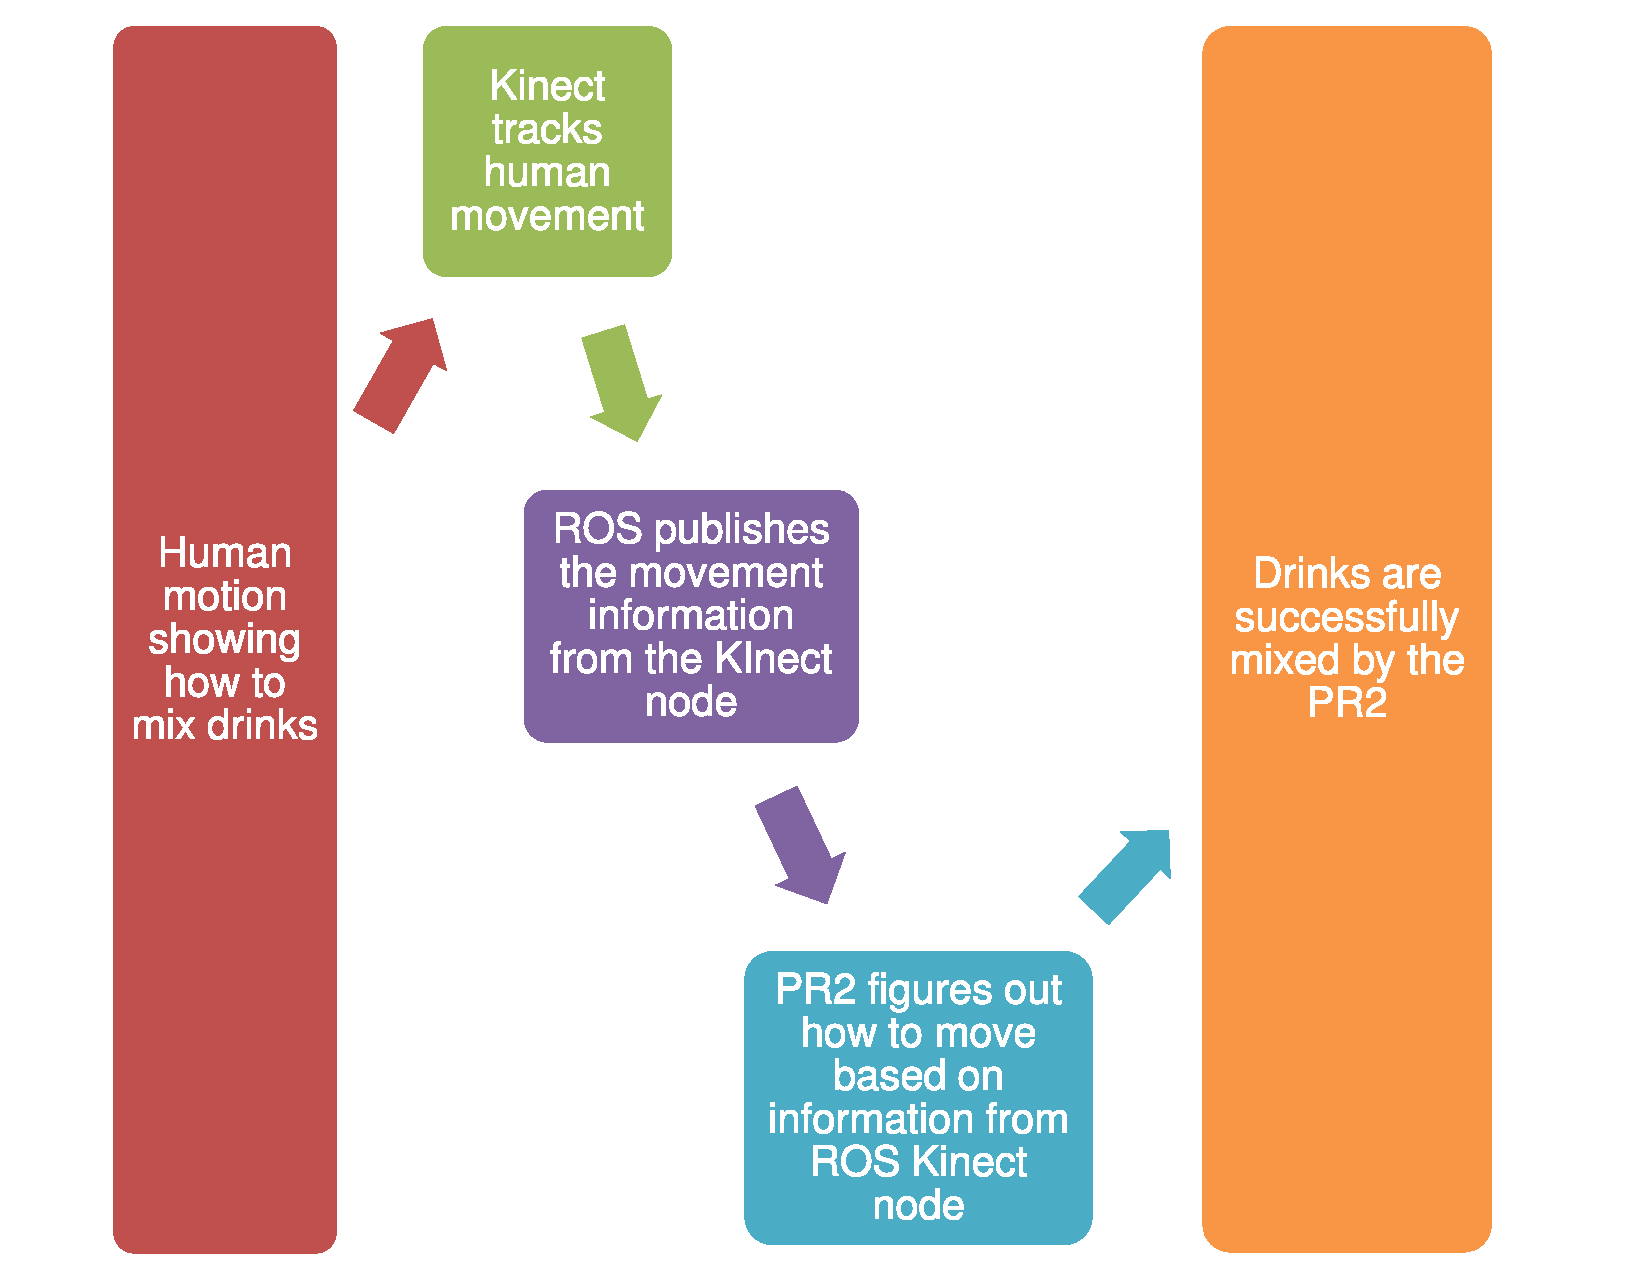
\includegraphics[width=1.0\linewidth]{flowchart}
	\end{center}
	%\vspace{-24pt}
	\caption{Block Diagram Summarizing System Model}
	\label{fig:some_graph}
\end{figure}
\section{System Implementation}

\section{Project Proposal}

\label{sec:project_proposal}We propose to teach a PR2 robot how to mix drinks via
teleimmersive demonstration learning methods. One of our major goals is to have the PR2
be able to reproduce different drink mixing recipes acquired from watching
a human demonstrator perform them in the past.
Our other major goal involves having the PR2 adapt its behavior by learning from failed attempts.
Given a setting consisting of many different bottles and glasses, the PR2 should be able to 
distinguish and select the desired bottles and them pour them into glasses by
combining its stored library of known mixes with reinforcement learning techniques.\\
The most visible metric of success will be  how well the PR2
can perform as a bartender. We can determine how often the PR2
successfully serves a requested drink. It is important to note, however, that the real
measure of success is how well teleimmersive learning via Kinect can be used
for robots to acquire new motions and behaviors.
\subsection{Anticipated Approach}
\label{subsec:approach}
Our method consists of two phases. First the robot will shadow a human teacher,
remembering the actions so that it can subsequently try to reproduce them. For example,
the sequence of moves involved for mixing a martini will be different than the ones
involved in mixing a gin and tonic.
In the next part, the PR2 will then attempt to improve its execution of the learned motion through 
reinforcement learning. For instance, if we move a cup two centimeters away
from its expected position, and the PR2 fails to pick it up, it can try again 
by adjusting its recorded sequence of moves.\\
For the first part, we propose using teleimmersive operation to demonstrate
behavior to the PR2 so that it can imitate and reproduce these motions at a
later time. At the base level, the hardware layer of the PR2 will be managed 
by ROS. This will be combined with the Microsoft XBOX Kinect to capture human
motion and to provide the teleimmersive framework. The Kinect will provide nodes
that can publish motion capture data, which in turn can be subscribed to by nodes
controlling parts of the PR2.
In this way,the PR2 can observe a human trainer go
through the process of selecting bottles and pouring them into glasses. 
Specialized software will then attempt to map the motions of the human trainer
onto the motor system of the PR2.\\
The second phase utilizes software that lets the PR2 attempt to reproduce
the observed motions augmented by reinforcement learning techniques. In addition
to simply trying to replicate the motion in identical situations,
the PR2 will evaluate its own performance in changing environments. For instance, 
objects may placed in the exact same location as they were placed for the human demonstrator.
The end goal is for the PR2 to refine its acquired motions and adapt to new
situations via reinforcement learning techniques.\\
ROS is a fairly mature and ubiquitous piece of software that can take care of
many of the more sophisticated computational tasks (such as path planning, 
image segmentation, etc.) that we would otherwise have to devote significant 
amounts of time to developing.  
Likewise, we intend to make heavy use of the Kinect API, which comes with very
strong support for human joint detection. The Kinect has already been integrated with 
ROS with great success.
While we expect both ROS and Kinect to have relatively steep learning curves,
we do not anticipate these being the limiting factor in how much progress we
are able to achieve. 
Rather, we expect the area of novel difficulty to be the combining of these
two distinct systems into one coherent system which can be used for
teleimmersive learning.
\subsection{Evaluation Criteria}
\label{subsec:eval_criteria}
We will evaluate the performance of our proposed system to teach the PR2 by experimentally determining how quickly and easily the PR2
can acquire new behavior. We will start with very simple motions, such as simply lifting and pouring a single cup or bottle. Once the PR2 is capable of completing those actions after shadowing a human demonstrator, we can attempt to teach it increasingly complex sequences of mixing and pouring. We can measure the PR2's success rate in repeating a recorded movement over multiple trials. This success rate can be then be correlated with the complexity of the demonstrated command. The goal here is to show that many different movement sequences of varying difficulty can be taught to the PR2 using the same motion capturing setup from the Kinect.\\
If time permits, we also plan to evaluate the PR2's ability to adapt to variable conditions. For instance, we can measure how far a bottle can be moved from its expected position before the PR2 becomes unable to pick it up. The weight of the bottle can also be changed to see how well the PR2 can adapt to grasping nearly-full versus nearly-empty drink containers. The success rate of the PR2's drink mixing can be analyzed as a function of these variables (distance moved, weight of drinks, etc).
\subsection{Block Diagram}
\label{subsec:block_diagram}

\section{Remaining Work}
\label{sec:remaining_work}
The following is a list of milestones we hope to reach as the spring semester progresses.

	% The 'itemize' environment shown here, and its friend 'enumerate' (shown below), are used to create indented\bulleted\outline style lists.
\begin{itemize*}
	\item {\sc prior-to Feb.1}: Attempt real trials on the actual PR2.\vspace{3pt}
	\item {\sc prior-to Mar.1}: Achieve a simple, successful drink mixing with the PR2.\vspace{3pt}
	\item {\sc prior-to Apr.1}: Develop a more complex sequence of drink mixing with the PR2.\vspace{3pt}
	\item {\sc completion tasks}: Verify that the PR2 can successfully mix a drink. Conduct accuracy testing. Complete write-up.\vspace{3pt}
	\item {\sc if there's time} : Investigate ways to improve the PR2's ability to adapt and learn from different drink configurations.
\end{itemize*}

	% AW: We next move onto the bibliography.
\bibliographystyle{plain} % Please do not change the bib-style
\bibliography{progress_spec}  % Just the *.BIB filename

\end{document} 
